\documentclass{article}[a4paper]
\usepackage[a4paper, total={6.5in, 9.5in}]{geometry}
\usepackage{charter}
\usepackage{xcolor}
\usepackage{graphicx}
\usepackage{float}
\usepackage{listings}
\usepackage{amsmath}
\usepackage{amssymb}
\usepackage[hidelinks]{hyperref}

\lstset{
  language=Python,
  basicstyle=\ttfamily,
  keywordstyle=\color{blue},
  commentstyle=\color{gray},
  stringstyle=\color{red},
  showstringspaces=false,
  columns=fullflexible,
  breaklines=true
}

\title{
	\huge{\textbf{
		Assignment 01
	}}\\
	\Large{
		Learning from Data, Related Challenges, Linear Models for Regression
	}\\
	\large{\phantom{}}\\
	\large{
		submitted for
	}\\
	\LARGE{
		\textbf{EN3150 - Pattern Recognition}
	}\\
	\large{
		Department of Electronic and Telecommunication Engineering
	}
	\\
	\large{University of Moratuwa}
}

\author{
	\textbf{Udugamasooriya P. H. J.}\\
	220658U % \quad - \quad \href{https://github.com/pulasthi-u/en3160-assignment01}{GitHub}\\
}

\date{12 August 2025}

\allowdisplaybreaks

\begin{document}

	\maketitle

	\section{Impact of Outliers on Linear Regression}

	\begin{figure}[H]
		\centering
		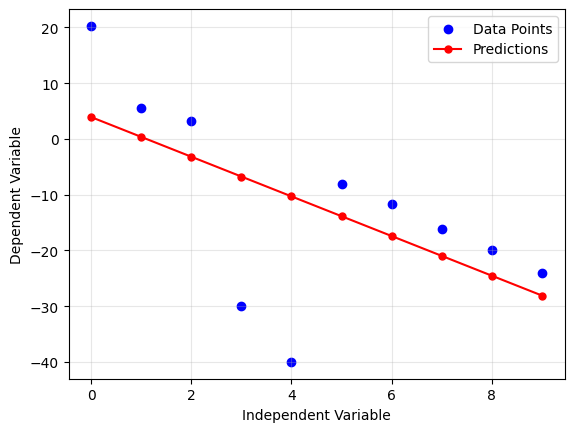
\includegraphics[width=0.8\linewidth]{images/q1.png}
		\caption{abc}
	\end{figure}

	\section{Loss Functions}

	\section{Data Pre-Processing}

\end{document}